\documentclass[11pt,letterpaper]{article}     % Tipo de documento y otras especificaciones
\usepackage[utf8]{inputenc}                   % Para escribir tildes y eñes
\usepackage[spanish]{babel}                   % Para que los títulos de figuras, tablas y otros estén en español
\usepackage[apaciteclassic]{apacite}
\usepackage{geometry}    
\usepackage{textcomp}
\geometry{left=25mm, right=25mm, top=25mm, bottom=25mm} % Tamaño del área de escritura de la página
\usepackage{amsmath}      % Los paquetes ams son desarrollados por la American Mathematical Society
\usepackage{amsfonts}     % y mejoran la escritura de fórmulas y símbolos matemáticos.
\usepackage{booktabs}
\usepackage{subfig}
\usepackage{amssymb}
\usepackage{graphicx}     % Para insertar gráficas
\usepackage{float}		% Para ubicar las tablas y figuras justo después del texto
\usepackage{pdfpages}
\batchmode
\usepackage{enumerate}
\usepackage{siunitx}
\pagestyle{plain} 
\usepackage{graphics}
\pagenumbering{arabic}
\usepackage{multicol}   % Para varias columnas
\usepackage{multirow}
\usepackage{color}%Paquete para colocar color al texto
%====================Español Venezolano Rápido============================
\renewcommand\tablename{Tabla}
\renewcommand\figurename{Figura}
%\renewcommand\prefacename{Prefacio}
\renewcommand\refname{REFERENCIAS}
%\renewcommand\bibname{REFERENCIAS}
\renewcommand\abstractname{Resumen}
%\renewcommand\chaptername{CAPÍTULO}
\renewcommand\appendixname{Apéndice}
\renewcommand\contentsname{ÍNDICE GENERAL}
\renewcommand\listfigurename{LISTA DE FIGURAS}
\renewcommand\listtablename{LISTA DE TABLAS}
\renewcommand\indexname{Índice Alfabético}
\renewcommand\partname{Parte}

%\renewcommand\enclname{Adjunto}
%\renewcommand\ccname{Copia a}
%\renewcommand\headtoname{A}
%\renewcommand\pagename{Página}
%\renewcommand\seename{véase}
%\renewcommand\alsoname{véase también}
%\renewcommand\proofname{Demostración}
%\renewcommand\glossaryname{Glosario}
%===================  Español venezolano =====================


\author{\\Omaña Enderson CI:  24.757.361 \\Raven Guillermo CI: 25.476.227\\Profesor: Crespo Jorge \vspace*{1in}}
\title{Universidad Central de Venezuela\\{ Facultad de Ingeniería\\Escuela de Ingeniería Eléctrica\\ Conversión Electromecánica de la energía\\\vspace*{1.5in} }Laboratorio 8\\MAQUINAS ASINCRÓNICAS O DE INDUCCIÓN\vspace*{1.35in}}
\date{Caracas, \today}

\begin{document}	% Inicio del documento
\maketitle							% Título
\newpage
\tableofcontents
\newpage
\section{Objetivos}
\begin{itemize}
	\item Presentar los métodos de medición y las condiciones de ensayos mínimas necesarias para la realización de las pruebas de laboratorio que son base para la determinación del circuito equivalente convencional.
	\item Deducir las ecuaciones matemáticas para la determinación de los parámetros del circuito equivalente.
	\item Determinar las curvas características más importantes de las máquinas de corriente continua.
    \item Presentar los algoritmos de los métodos iterativos para la determinación y ajuste del circuito equivalente, respectivamente.
    \item Comprobar a través de determinaciones, la validez de los métodos presentados para la obtención del circuito equivalente de una maquina de inducción.
\end{itemize}
\section{Marco Teórico}
\subsection{Método A}
Se usa para maquinas cuyo ensayo de rotor trabado fue realizado con tensiones de frecuencia menor al valor nominal, tal que: 
\begin{equation}
	f_{cc}\approx 25\%f_{nom}
\end{equation}
Estos son los pasos a seguir del método:
\begin{enumerate}
	\item Se deben conocer la tensión y corriente por fase, en el estátor consumida durante la prueba de vacío $V_{1,0}$ y $I_{1,0}$. La potencia por fase consumida por la maquina en vacío $P_{1,0}$. Tensión y corriente por fase, en el estátor consumida durante la prueba de rotor trabado, $V_{1,cc}$ y $I_{1,cc}$ y la potencia por fase consumida por la maquina durante el ensayo de rotor trabado, $P_{1,cc}$.
	\item Asumir un valor de $X_{1}$/$X_{2}$. En los casos que no se disponga de esta información tomar en cuenta los valores sugeridos en el estándar IEEE 112, segun el código ó ``Letra diseño" NEMA de la maquina:
	\begin{itemize}
		\item Diseño NEMA A,D y rotor bobinado: $X_{1}$/$X_{2}$ = 1.
		\item Diseño NEMA B: $X_{1}$/$X_{2}$ = 0,67.
		\item Diseño NEMA C: $X_{1}$/$X_{2}$ = 0,43.
	\end{itemize}
	\item Asumir un valor inicial de la reactancia de magnetización $X_{m,0}$ y estatórica de dispersión $X_{1,0}$. 
	
	Se toman como valores iniciales los valores obtenidos en las pruebas de vacío y rotor trabado de modo que quedarían las siguientes expresiones:
	\begin{align}
		X_{1_{(0)}} = \frac{\sqrt{\left(\frac{V_{1,cc}}{I_{1,cc}}\right)^{2}-\left(\frac{P_{1,cc}}{I_{1,cc}^{2}}\right)^{2}}}{1+\frac{X_{2}}{X_{1}}}\label{X10equ}\\
		X_{m_{(0)}} = \left\|\frac{\overline{V_{1,0}}}{\overline{I_{1,0}}}-(R_{1}+jX_{1,(i)})\right\| \label{Xm0equ}
	\end{align}
	\item Calcular $Q_{1,0}$ y $Q_{1,cc}$ respectivamente mediante:
	\begin{align}
		Q_{1,0} = \sqrt{(V_{1,0}\cdot I_{1,0})^{2}-P_{1,0}^{2}} \label{Q10equ}\\
		Q_{1,cc} = \sqrt{(V_{1,cc}\cdot I_{1,cc})^{2}-P_{1,cc}^{2}} \label{Q1ccequ}
	\end{align}
	\item Calcular $X_{m,(i+1)}$:
	\begin{equation}
		X_{m,(i+1)} = \frac{V_{1,0}^{2}}{Q_{1,0}-I_{1,0}^{2}\cdot X_{1,(i)}}\cdot \frac{1}{\left(1+\frac{X_{1,(i)}}{X_{m,(i)}}\right)^{2}}\label{Xm(i+1)equ}
	\end{equation}
	\item Calcular $X_{1,cc,(i)}$:
		\begin{equation}
	X_{1,cc,(i)} =  \frac{Q_{1,cc}}{I_{1,cc}^{2}\cdot\left(1+\frac{X_{1}}{X_{2}}+\frac{X_{1,(i)}}{X_{m,(i)}}\right)}\cdot\left(\frac{X_{1}}{X_{2}}+\frac{X_{1,(i)}}{X_{m,(i)}}\right) \label{X1cciequ} 
	\end{equation}
	\item Calcular $X_{1,(i+1)}$:
	\begin{equation}
		X_{1,(i+1)} = \frac{f_{nom}}{f_{cc}}X_{1,cc,(i)} \label{X1(i+1)equ}
	\end{equation}
	\item Para i = i+1 repetir paso 5 hasta el paso 7 hasta que los valores de las reactancias de dispersión y mutua se estabilicen alrededor de un 0,1\% de diferencia; es decir:
	\begin{align}
		|X_{1,(i+1)}-X_{1,(i)}| \leq 0,001 \label{esperadoX1}\\
		|X_{m,(i+1)}-X_{m,(i)}| \leq 0,001 \label{esperadoXm}
	\end{align}
	\item Calcular $X_{2}$:
	\begin{equation}
		X_{2} = \frac{X_{1,(i+1)}}{\frac{X_{1}}{X_{2}}} \label{X2equ}
	\end{equation}
	\item Determinar gráficamente y a partir de las mediciones realizadas el valor de las perdidas mecánicas $P_{mec}$.
	\item Calcular $P_{fe}$:
	\begin{equation}
		P_{fe} = P_{1,0}-\frac{P_{mec}}{3}-I_{1,0}^{2}\cdot R_{1} \label{Pfe}
	\end{equation}
	\item Calcular $g_{fe}$:
	\begin{equation}
		g_{fe} = \frac{P_{fe}}{V_{1,0}^{2}}\left(1+\frac{X_{1,(i+1)}}{X_{m,(i+1)}}\right)^{2} \label{gfeequ}
	\end{equation} 
	\item Calcular $R_{fe}$:
	\begin{equation}
	R_{fe} = \frac{1}{g_{fe}} \label{Rfe}
	\end{equation}
	\item Calcular $R_{2}$:
	\begin{equation}
		R_{2} = \left(\frac{P_{cc}}{I_{1,cc}^{2}}-R_{1}\right)\left(1+\frac{X_{2}}{X_{m,(i+1)}}\right)^{2}-\frac{X_{2}^{2}}{X_{1,(i+1)}^{2}}\cdot X_{1,cc,(i)}^{2}\cdot g_{fe} \label{R2equ}
	\end{equation}
\end{enumerate}

\section{Lista de instrumentos}
\begin{table}[H]
	\caption{Lista de instrumentos de medición y componentes}
	\centering
	\begin{tabular}{|c|c|}
		\hline 
		Instrumento & Alcance ó especificaciones \\ \hline 
		Vatimetro &  fp = 0,2 \\  
		\hline 
		Vatimetro &  fp Alto\\  
		\hline 
		Reostato &  (0-33) $\Omega$; 4.2 A \\  
		\hline
		Termometro ó Termocupla &  - \\  
		\hline
		Transformador de corriente &  - \\  
		\hline
		Reostato &  (0-100) $\Omega$; 2.4 A \\  
		\hline
		Voltímetros de bobina móvil y hierro móvil &  (0-150) V/ (0-15) V/(0-30) V/(0-300) V\\  
		\hline 
		Multímetro CEN-TECH & -\\  
		\hline 
		Resistencia de shunt & (En laboratorio se determinaran)\\  
		\hline
		Tacometro & -\\  
		\hline
		Carga lineal & 200 w, 400w, 800w, 1kw\\  
		\hline
		Amperímetro de bobina móvil y hierro móvil &(0-1.2) A/ (0-6) A/(0-30) A \\ 
		\hline
		Protecciones AC & 25 A; 380 V\\ 
		\hline
		Protecciones DC & -\\ 
		\hline
		\multirow{5}{3cm}{Motor AC} & - V \\ 
		\cline{2-2}
		& - A  \\
		\cline{2-2}
		& - rpm\\
		\cline{2-2}
		&- hp\\
		\cline{2-2}
		&carga -\%\\
		\hline
		\multirow{5}{3cm}{Generador DC} & 3 KV\\ 
		\cline{2-2}
		& 125 V \\
		\cline{2-2}
		&26,5 A\\
		\cline{2-2}
		& 1000 rpm\\
		\hline
		
		
	\end{tabular} 
\end{table}
\section{Condiciones de ensayo}
Estas son las precauciones y normativas necesarias para realizar el laboratorio de forma segura y efectiva: 
\begin{itemize}
    \item \textbf{Respecto a la prueba de vacío con rotor cortocircuitado:} La máquina a la que se le hará la prueba deberá estar conectada como motor. Es necesario tener especial cuidado de no seguir reduciendo la tensión cuando la maquina comience elevar la corriente, debido a que esto puede causar el colapso de la maquina.
   
    Es recomendable que los vatímetros posean un factor de potencia bajo.
    \item \textbf{Respecto a la medición de resistencia estatórica:} Se trabajara asegurándose que la corriente máxima alcanzada sea menor o igual al 10 \% de la corriente nominal. La resistencia obtenida deberá ajustarse de acuerdo a la temperatura.
    \item \textbf{Respecto a la prueba de rotor trabado:} Se debe tener especial cuidado en las cercanías de la carga completa, debido a las corrientes que se pueden alcanzar, por este motivo se trabajara a tensión reducida con un vatímetro preferiblemente de alto factor de potencia, se recomienda registrar  la temperatura del devanado del estátor o la resistencia del devanado del mismo.
    
    Se debe tener cuidado de no sobre calentar los devanados. Tomando las lecturas más altas primero y las lecturas más bajas en sucesión (Según IEEE Std 112-2004). Ayudará a igualar la temperatura.
    \item \textbf{Respecto a la medición de la curva de carga:} Se debe medir a velocidad constante.
    \item \textbf{Respecto a la  vestimenta:} No usar franelas o camisas manga larga, llevar zapatos de goma y pantalones. No usar collares ni pulseras de metal.
    \item \textbf{Previo a las pruebas:} Hacer primero el montaje antes de energizar, al culminarlo preguntar al profesor si las conexiones son correctas para proceder con las pruebas.
    \item \textbf{Respecto a la comunicación:} Mantener informado sobre cualquier cambio en el montaje al compañero de laboratorio y por sobre todo informar si el circuito se encuentra energizado o no.
	\item \textbf{Respecto a las curvas observadas:} No aceptar como adecuada una curva que este llena de ruido, ya que se puede deber a que algún elemento puede estar actuando como antena, esto originara incertidumbre en los resultados.
	\item \textbf{Respecto al numero de mediciones:}
	Realizar al menos 5 mediciones para condiciones distintas.
	\item \textbf{Respecto a la elección de componentes y las conexiones:} Evitar los componentes que puedan funcionar como antenas (como resistencias de shunt de tipo mariposa u algún otro que se encuentre muy expuesto) y cuidar los contactos de cada conexión.
    \item \textbf{Respecto a la manipulación:} En caso de maniobrar el circuito energizado manipular con la mano derecha, buscando mayores probabilidades de sobrevivir en caso de un accidente eléctrico.
\end{itemize}
\section{Procedimiento}
\subsection{Medición de resistencia estatórica}
\begin{enumerate}
	\item Lo primero sera, hallar las resistencias internas por fase, por lo que se realizaran las conexiones como en la Figura \ref{fig:modeloConexionResistencias}.
	\item Se alimentaran las fases del estátor con tensión DC a una fracción de la tensión nominal.
	\item Manteniendo la tensión fija, se irá ajustando el variac, se tomara nota de los valores de tensión y corriente (en caso de ser muy elevada la corriente, se colocara una resistencia de shunt para realizar la medición) en cada fase. Se tomaran al menos 4 mediciones por cada fase.
	\item Se verificara si la conexión del estátor se encuentra en delta o en estrella, ya que de ser delta la resistencia por fase sera:
	\begin{equation}
	R_{fase} = \frac{V_{DC_{\phi}}}{2\cdot I_{DC_{\phi}}}
	\end{equation} 
	En delta sera:
	\begin{equation}
	R_{fase} = \frac{3\cdot V_{DC_{\phi}}}{2\cdot I_{DC_{\phi}}}
	\end{equation} 
	\item Se des-energizara el circuito.
\end{enumerate}
\subsection{Prueba en vacío con rotor cortocircuitado}
\begin{enumerate}
	\item Se armara el circuito presente en la Figura \ref{fig:diagramaDeConexion}, sin conectar carga alguna. Es importante denotar que para cada medición se tomara nota de la tensión  de linea, corriente de linea y potencia.
	\item Se iniciaran las mediciones desde donde rompa la inercia inicial el motor hasta la tensión nominal y se ira bajando en pasos equidistantes hasta que la corriente en vez de bajar comience a subir.
\end{enumerate}
\subsection{Prueba de rotor trabado}
\begin{enumerate}
	\item Se trabara mecánicamente el motor. Es importante denotar que para cada medición se tomara nota de la tensión  de linea, corriente de linea y potencia.
	\item Se realizara al menos una medición mientras el rotor se encuentra trabado, se espera que la corriente sea la nominal y la potencia activa.
\end{enumerate}
\subsection{Efecto de carga}
\begin{enumerate}
	\item Al circuito de la Figura \ref{fig:diagramaDeConexion} se le conectara un generador sincronico y este se conectara a una carga con el fin de visualizar el efecto de carga. Es importante denotar que para cada medición se tomara nota de la tensión  de linea, corriente de linea y potencia.
	\item Se medirán los parámetros para distintas cargas conectadas al generador DC alimentado por el motor AC (al menos 4).
\end{enumerate}
\section{Diagramas}

	\begin{figure}[H]
	\centering
	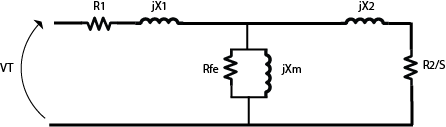
\includegraphics[scale=0.8]{./recursos-Lab8/modeloInternoMotorInduccion.png}
	\caption{Modelo de motor de inducción}
	\label{fig:modeloMotorInduccion}
\end{figure}

\begin{figure}[H]
	\centering
	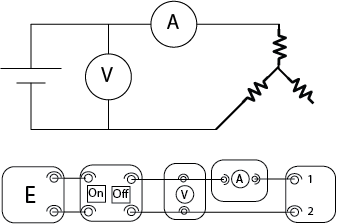
\includegraphics[scale=0.8]{./recursos-Lab8/diagramaConexionMedicionResistencia.png}
	\caption{Diagrama circuital y de conexion de medición de resistencias internas}
	\label{fig:modeloConexionResistencias}
\end{figure}

\begin{figure}[H]
	\centering
	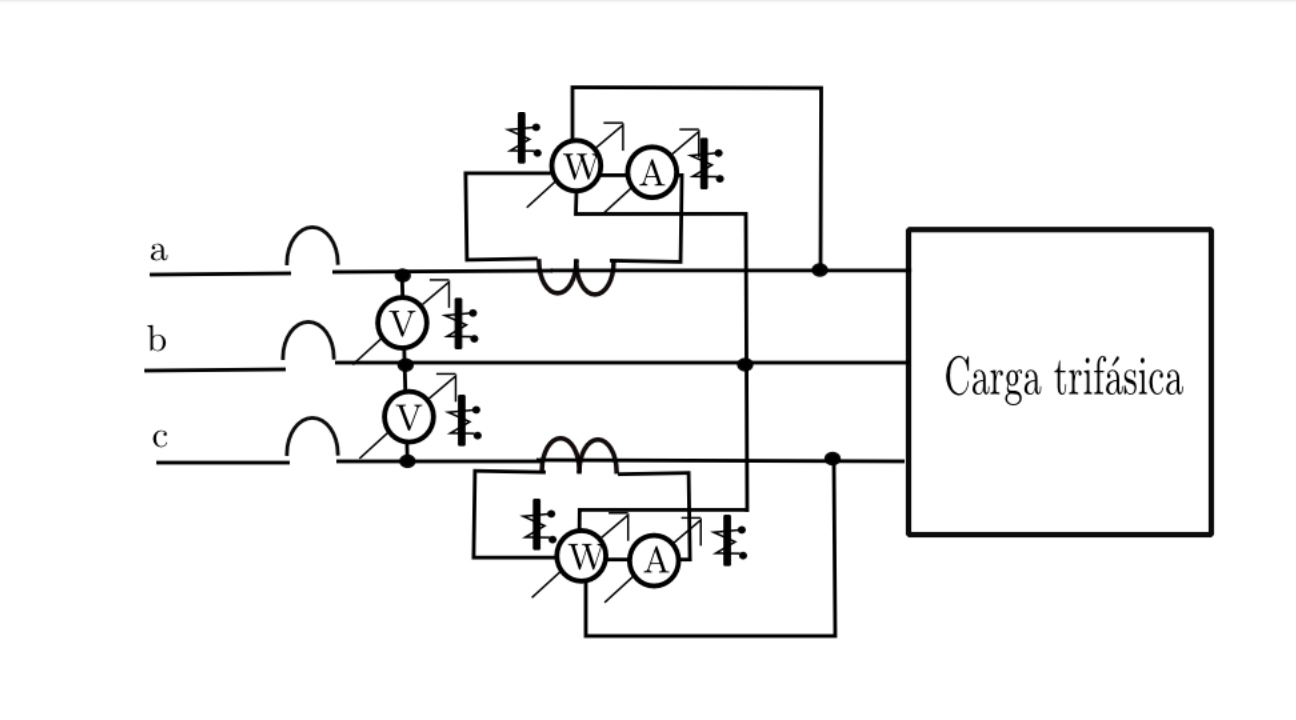
\includegraphics[scale=0.2]{./recursos-Lab8/diagramaCircuitalmedicionPotenciaVoltajeCorriente.jpg}
	\caption{Diagrama circuital de la conexión voltímetro, amperímetro y vatímetro}
	\label{fig:diagramaDeConexion}
\end{figure}


\section{Resultados}
\subsection{Medición de resistencia interna}
Para obtener el valor de R1 del Cuadro \ref{cuadro medicion de resistencia} se calculan los promedios de cada grupo de medidas:
\begin{table}[H]
	\centering
	\caption{Resultados medición de resistencia}
	\label{cuadro medicion de resistencia}
	\begin{tabular}{|c|c|c|c|c|c|c|c|}
		\hline
		$V_{10-11} [V]$ &$ V_{11-12} $[V] &$ V_{12-10}$ [V] &$ I_{10}$ [A] & $I_{11}$ [A] &$ I_{12}$ [A] &$ V_{promedio}$ & $I_{promedio}$ \\ \hline
		1,50 $\pm$ 0,02 & 0,58$\pm$0,02 & 1,40$\pm$0,02 & 0,82$\pm$0,02 & 0,84$\pm$0,02 & 0,82$\pm$0,02 & 1,16$\pm$0,02 & 0,83$\pm$0,02 \\ \hline
		1,50$\pm$0,02 & 0,62$\pm$0,02 & 1,60$\pm$0,02 & 1,0$\pm$0,1 & 1,0$\pm$0,1 & 1,0$\pm$0,1 & 1,24$\pm$0,02 & 1,0$\pm$0,1 \\ \hline
		1,70$\pm$0,02 & 0,80$\pm$0,02 & 1,70$\pm$0,02 & 1,3$\pm$0,1 & 1,3$\pm$0,1 & 1,3$\pm$0,1 & 1,4$\pm$0,02 & 1,3$\pm$0,1 \\ \hline
		1,90$\pm$0,02 & 1,14$\pm$0,02 & 2,00$\pm$0,02 & 1,7$\pm$0,1 & 1,7$\pm$0,1 & 1,7$\pm$0,1 & 1,68$\pm$0,02 & 1,7$\pm$0,1 \\ \hline
		2,20$\pm$0,02 & 1,38$\pm$0,02 & 2,20$\pm$0,02 & 2,0$\pm$0,1 & 2,0$\pm$0,1 & 2,0$\pm$0,1 & 1,92$\pm$0,02 & 2,0$\pm$0,1 \\ \hline
	\end{tabular}
\end{table}

Epleando los valors del cuadro \ref{cuadro medicion de resistencia} se linealizó mediante míimos cuadrados y se obtuvo lo siguiente:

	\begin{figure}[H]
	\centering
	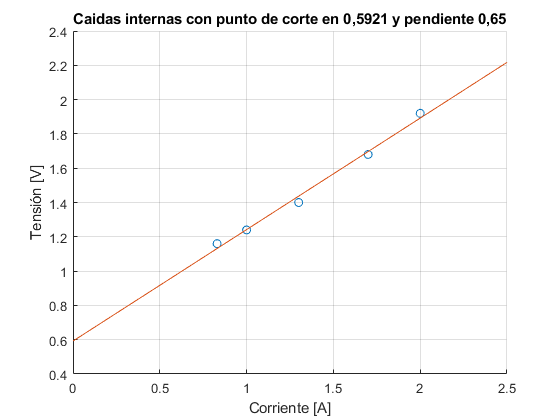
\includegraphics[scale=0.8]{./recursos-Lab8/curvaPruebasDeResistenciaInterna.png}
	\caption{Recta obtenida por regresión lineal correspondiente a la resistencia interna}
	\label{fig:rectaResistenciaInterna}
\end{figure}
Para calcular la incertidumbre asociada a la pendiente hallada se determino la desviación estandar:
\begin{equation}
\sigma = \sqrt{\frac{\sum_{i=1}^{N}(y_{i}-m\cdot x_{i}-b)^{2}}{N-2}} \label{desvEstandar}
\end{equation}
Donde:\\
N: numero de datos\\
b: Punto de corte obtenido\\
m: Pendiente obtenida\\
$y_{i}$: Datos del eje y\\
$x_{i}$: Datos del eje x

Utilizando la desviación se calcula incertidumbre de la pendiente mediante la siguiente ecuación:
\begin{equation}
\Delta m = \sigma \sqrt{\frac{N}{N\sum_{i=1}^{N}x_{i}^{2}-\left(\sum_{i=1}^{N}x_{i}\right)^{2}}} \label{incertiPendiente}
\end{equation}

Por lo tanto la resistencia de campo medida sera: $R_{estatorica(medida)}$ = 0,65 $\pm$ 0,0269 $\Omega$. No obstante se requiere ajustar el valor respecto a la temperatura empleando la siguiente expresión:
\begin{align}
R_{estatorica} = R_{(medida)} \frac{T_{r}+T_{k}}{T_{m}+T_{k}} \label{ajusteTemp}
\end{align}
Donde:\\
$T_{k}$ : 234.5 \textdegree C (cobre).\\
$T_{m}$ : Temperatura a la cual se midió la resistencia, 25 \textdegree C.\\
$T_{r}$ : Es la temperatura de referencia en \textdegree C (75 \textdegree C).\\

Entonces: $R_{estatorica(ajustada)}$ = 0,775 $\pm$ 0,0269 $\Omega$, ya que la conexión del motor es en estrella la $R_1=R_{estatorica}/2 = 0,3875 \pm 0,0269 \Omega$ 
\subsection{Prueba de vacío}
\begin{table}[h]
	\centering
	\caption{Datos experimentales prueba de vacío}
	\label{tabla:resultadosPruebasVacio}
	\begin{tabular}{|c|c|c|c|c|c|}
		\hline
		\textbf{$V_{10-11}$ [V]} & \textbf{$V_{11-12}$ [V]} & \textbf{$V_{12-10} $[V]} & \textbf{$I_{10} $[A]} & \textbf{$P_1$[W]} & \textbf{$P_2[W]$} \\ \hline
		87 $\pm$ 1 & 85$\pm$1 & 87$\pm$1 & 6,5$\pm$0,5 & 520$\pm$10 & -250$\pm$10 \\ \hline
		108$\pm$1 & 107$\pm$1 & 108$\pm$1 & 5,5$\pm$0,5 & 580$\pm$10 & -190$\pm$10 \\ \hline
		128$\pm$1 & 127$\pm$1 & 127$\pm$1 & 4,5$\pm$0,5 & 620$\pm$10 & -130$\pm$10 \\ \hline
		148$\pm$2 & 146$\pm$2 & 148$\pm$2 & 4,5$\pm$0,5 & 710$\pm$10 & -50$\pm$10 \\ \hline
		166$\pm$2 & 166$\pm$2 & 168$\pm$2 & 5,0$\pm$0,5 & 780$\pm$10 & 50$\pm$10 \\ \hline
		184$\pm$2 & 184$\pm$2 & 186$\pm$2 & 5$\pm$0,5 & 870$\pm$10 & 130$\pm$10 \\ \hline
		204$\pm$2 & 204$\pm$2 & 206$\pm$2 & 5,5$\pm$0,5 & 1020$\pm$10 & 240$\pm$10 \\ \hline
	\end{tabular}
\end{table}
Con los valores del cuadro \ref{tabla:resultadosPruebasVacio} se realiza la curva de $P_{3\phi}$ respecto a $V_{\phi}^2$ cuyo corte con el eje nos da el valor de las perdidas mecanicas del rotor, para ello construimos el cuadro \ref{cuado: p3f y Vf} donde:
\begin{eqnarray}
V_{\phi}=\frac{V_{L1}+V_{L2}+V_{L3}}{3\sqrt{3}}\\
\Delta V_{\phi}= \bigg|\frac{\delta V_{\phi}}{V_{Li}}\bigg| \cdot \Delta V_{Li} = \frac{\Delta V_{L1}+\Delta V_{L2}+\Delta V_{L3}}{3 \sqrt{3}}
\end{eqnarray}
Ya que se empleo el metodo de los 2 vatímetros la potencia total viene dada por:
\begin{eqnarray}
P_{total}=P_1+P_2\\
\Delta P_{total}=  \bigg|\frac{\delta P_{total}}{P_1}\bigg| \cdot \Delta P_1 + \bigg|\frac{\delta P_{total}}{P_2}\bigg| \cdot \Delta P_2 = \Delta P_1 + \Delta P_2
\end{eqnarray}

\begin{table}[H]
	\centering
	\caption{Cuadro de potencia total y tensión de fase promedio}
	\label{cuado: p3f y Vf}
	\begin{tabular}{|c|c|}
		\hline
		$P_{total}$[W]&$V_{\phi}promedio [V]$ \\ \hline
		270 $\pm$20&49,84$\pm$ 0,57\\ \hline
		390 $\pm$20&62,16$\pm$0,57 \\ \hline
		490 $\pm$20&73,51$\pm$0,57 \\ \hline
		660$\pm$20&85,06$\pm$1,14 \\ \hline
		830$\pm$20&96,22$\pm$1,14 \\ \hline
		1000$\pm$20&106,62$\pm$1,14 \\ \hline
		1260$\pm$20 & 118$\pm$1,14 \\ \hline		
	\end{tabular}
\end{table}

Para obtener el valor de $P_{3\phi}$ los vatímetros se encontraban restándose, empleando las ecuaciones \ref{desvEstandar} y \ref{incertiPendiente} con la regresión lineal se obtiene:

\begin{figure}[H]
	\centering
	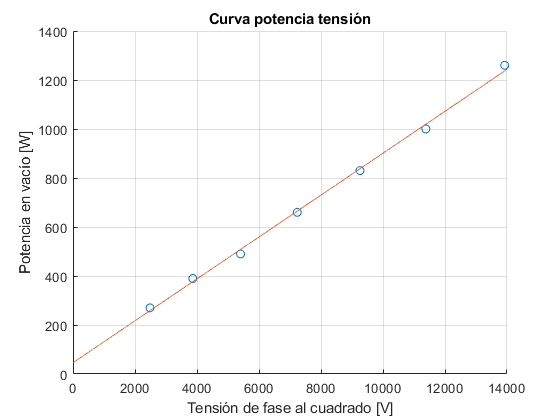
\includegraphics[scale=0.8]{./recursos-Lab8/curvaPruebaVacioPotenciaVsTensionCuadrado.png}
	\caption{Curva potencia tensión de fase cuadrado}
	\label{fig:curvaPotenciaTensionCuadrado}
\end{figure}

El corte con el eje el cual representa las pérdidas mecánicas valen $P_m=46,30\pm 0,11$ W.
\subsection{Prueba de rotor trabado}
Por medición indirecta al plantear las siguientes ecuaciones obtenemos:
\begin{eqnarray}
V_{\phi}=\frac{V_L}{\sqrt{3}}\\
\Delta V_{\phi}= \bigg|\frac{\delta V_{\phi}}{V_L}\bigg| \cdot \Delta V_L = \frac{\Delta V_L}{\sqrt{3}}
\end{eqnarray}

Utilizando lo calculado mediante la expresión previa y 
los datos experimentales se armo el siguiente cuadro:
\begin{table}[H]
	\centering
	\label{rotorTrabado}
	\caption{prueba de rotor trabado}
	\begin{tabular}{|c|c|c|c|c|c|}
		\hline
		$V_L$[V]&$V_{\phi}[V]$& $I_{\phi}[A]$ & $P_1$[W]&$P_2$[W]&$P_{total}$[W]\\ \hline
		41$\pm$1& 23,67$\pm$0,57&12,5$\pm$0,5&90$\pm$5&5$\pm$5& 95$\pm$10\\ \hline
	\end{tabular}
\end{table}
Cabe destacar que la corriente fue medida luego de pasar por un transformador de corriente.
\subsection{Método A}
\subsubsection{Paso 1}
De acuerdo a las mediciones previas los parámetros iniciales son los siguientes:
\begin{itemize}
	\item $V_{1,0}$: corresponde con el ultimo valor del cuadro \ref{cuado: p3f y Vf}, sería (118 $\pm$ 1,14) V.
	\item $I_{1,0}$: corresponde con el ultimo valor del cuadro \ref{tabla:resultadosPruebasVacio}, sería (5,5 $\pm$ 0,5) A.
	\item $P_{1,0}$: corresponde con el ultimo valor del cuadro \ref{cuado: p3f y Vf} entre 3, sería (420 $\pm$ 20) W.
	\item $V_{1,cc}$:  (23,67 $\pm$ 0,57) V.
	\item $I_{1,cc}$: (12,5 $\pm$ 0,5) A.
	\item $P_{1,cc}$: (31,66 $\pm$ 10) W.
\end{itemize}
\subsubsection{Paso 2}
Se asumirá un diseño de NEMA A ó D, por lo tanto $X_{1}$/$X_{2}$ = 1.
\subsubsection{Paso 3}
Empleando las ecuaciones \ref{X10equ} y \ref{Xm0equ} se tiene que:
\begin{itemize}
	\item $	X_{1_{(0)}} = 0,9414$ $\Omega$ .
	\item $X_{m_{(0)}} =21,7353$ $\Omega$ .
\end{itemize}
\subsubsection{Paso 4}
Con las ecuaciones \ref{Q10equ} y \ref{Q1ccequ} se obtiene:
\begin{itemize}
	\item $	Q_{1,0} = 494,7737 $ W.
	\item $Q_{1,cc} = 294,1762$ W.
\end{itemize}
\subsubsection{Pasos 5,6,7 y 8}
Aplicando el metodo mediante un algoritmo hecho en matlab se obtiene lo siguiente:
\begin{table}[H]
	\centering
	\caption{Pasos 5, 6, 7 y 8 (Resultados)}
	\label{MetodoAItera}
	\begin{tabular}{|c|c|c|c|c|}
		\hline
		\textbf{i} & \textbf{X\_\{m\} {[}$\Omega${]}} & \textbf{X\_\{1\} {[}$\Omega${]}} & \textbf{$|X_{m,(i+1)}-X_{m,(i)}|$} & \textbf{$|X_{1,(i+1)}-X_{1,(i)}|$} \\ \hline
		0          & 21,7353                          & 0,9414                           & -                                  & -                                  \\ \hline
		1          & 27,4330                          & 0,9613                           & 5,6978                             & 0,02                               \\ \hline
		2          & 27,9092                          & 0,9576                           & 0,4762                             & 0,0037                             \\ \hline
		3          & 27,9419                          & 0,9572                           & 0,0327                             & 0,0003                             \\ \hline
		4          & 27,9441                          & 0,9572                           & 0,0022                             & 0                                  \\ \hline
		5          & 27,9443                          & 0,9572                           & 0,0001                             & 0                                  \\ \hline
	\end{tabular}
\end{table}

De acuerdo con el cuadro previo $X_{m}$ es 27,9443 $\Omega$ y $X_{1}$ 0,9572 $\Omega$ .
\subsubsection{Paso 9}
Dado que que $X_{2}$ = $X_{1}$ entonces este sera 0,9572 $\Omega$.
\subsubsection{Paso 10}
Este paso se realizo previamente y se obtuvo que las $P_{mec}$ son (46,30 $\pm$ 0,11) W.
\subsubsection{Paso 11}
Aplicando la ecuación \ref{Pfe} se tiene que $P_{fe}$ = 392,8448 W.
\subsubsection{Paso 12}
Aplicando la ecuación \ref{gfeequ} se tiene que $g_{fe}$ = 0,0302 $\Omega^{-1}$.
\subsubsection{Paso 13}
Aplicando la ecuación \ref{Rfe} se tiene que $R_{fe}$ = 33,1351 $\Omega$.
\subsubsection{Paso 14}
Aplicando la ecuación \ref{R2equ} se tiene que $R_{2}$ = 0,2081 $\Omega$.
\section{Modelo obtenido} 
\newpage
\section{Análisis de resultados}
Se comprueba que efectivamente la reactancia por los flujos dispersos es mucho más grande que las reactancias en los arrollados, además la resistencia en el núcleo es al menos 30 veces la estatórica sumada a la resistencia en el rotor, de modo que las perdidas en el núcleo son mayores a las perdidas en cortocircuito en un factor entre 3 y 4 veces. Por estos motivos no es de extrañar que la maquina en vació posee mayores perdidas que a motor trabado, ya que en vació prácticamente la mayoría de las perdidas se deben al núcleo, debido a que las perdidas en el cobre del estátor son realmente mínimas. Mientras que en cortocircuito las perdidas del núcleo son ignoradas debido a la mínima corriente que circula por el mismo.
\newpage
\section{Conclusión}
El caracterizar una maquina asincrónica es sencillo a nivel experimental, pero para calcular los parámetros, a menos que se posea el algoritmo completo de alguno de los métodos de calculo de parámetros, puede volverse una tarea larga incluso el programar dicho algoritmo en algún software de calculo, ya que la cantidad de ecuaciones que maneja el método es considerable. El método A no es algo que sea recomendable para realizar a mano ya que la probabilidad de equivocarse en alguna cuenta es realmente elevada, por este motivo se recomienda realizar una función u algún programa que ejecute todos los pasos necesarios para obtener los resultados deseados.
\newpage
\section{Anexos}
\begin{figure}[H]
	\centering
	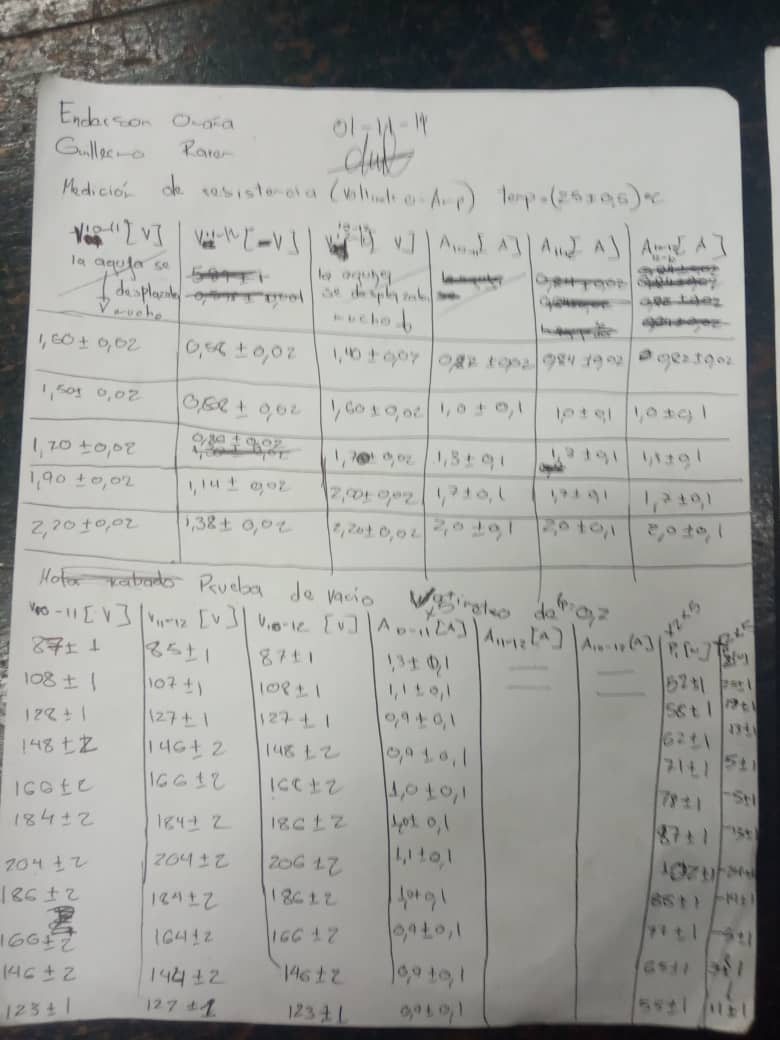
\includegraphics[scale=0.55]{./recursos-Lab8/HojaDeDatos1.jpeg}
	\caption{Hoja de datos 1}
\end{figure}
\begin{figure}[H]
	\centering
	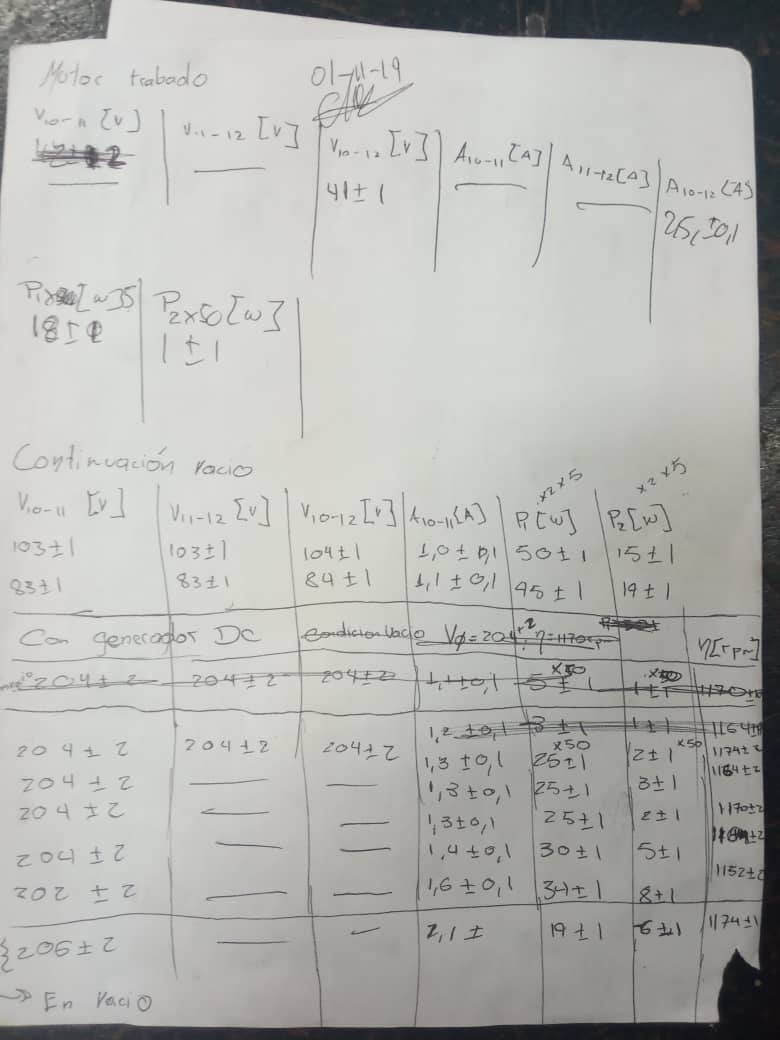
\includegraphics[scale=0.6]{./recursos-Lab8/HojaDeDatos2.jpeg}
	\caption{Hoja de datos 2}
\end{figure}
\end{document}
